\documentclass[twocolumn]{article}[9pt]
% \usepackage[utf8]{inputenc}%
% \usepackage{tikz}
% \usepackage{cfr-lm}%
\usepackage{jmlr2e}
\usepackage[T1]{fontenc}%
% \usepackage{physics}
\usepackage{amsmath}
\usepackage{amssymb}
\usepackage{graphicx}
\usepackage[margin=2cm]{geometry}
% \usepackage{changepage}
\usepackage{fontspec}
\usepackage{minted}
\usepackage{tcolorbox}
\usepackage{lmodern}
\usepackage{xcolor}
\usepackage{nccmath}
\usepackage{lettrine}
\usepackage{cuted}
% \usepackage{fontawesome}
\usemintedstyle{bw}
\usepackage{hyperref}
\hypersetup{
    colorlinks=false, pdfborder={0 0 0}
}


\newcommand\blfootnote[1]{%
  \begingroup
  \renewcommand\thefootnote{}\footnote{#1}%
  \addtocounter{footnote}{-1}%
  \endgroup
}


\newtcbox{\codebox}[1][black]{on line, arc=2pt,colback=#1!10!white,colframe=white, before upper={\rule[-3pt]{0pt}{10pt}},boxrule=1pt, boxsep=0pt,left=2pt,right=2pt,top=1pt,bottom=.5pt}
% \definecolor{antwhite}{HTML}{323333}
\newcommand{\code}[3][]{\codebox{\mintinline[#1]{#2}{#3}}}

\title{Tittel}%
\author{Brage Wiseth}%
\date{\today}%

% \setmainfont{FreeSans}
% \setmainfont{SF Pro Display}
% \setmainfont{IBM Plex Sans}
% \setmainfont{TeX Gyre Heros}
% \setmainfont{Inter}
% \setmainfont{Iosevka Quasi}

\setmonofont[Scale=MatchLowercase]{DM Mono}
% \setmonofont[medium]{Jetbrains Mono}

\begin{document}%
% \maketitle%
% \normalfont
\begin{strip}%
    \begin{center}
        \textbf{\LARGE Image Classification with Fine-tuning of Pre-trained Models}
    \end{center}
    \vspace{0.5em}
    \begin{center}
        \textbf{Brage Wiseth}
    \end{center}
    \begin{center}
        \textbf{\today}
    \end{center}
    \vspace{0.5em}


% \begin{abstract}%   <- trailing '%' for backward compatibility of .sty file
% \lettrine{T}{}his paper describes the mixtures-of-trees model, a probabilistic 
% model for discrete multidimensional domains.  Mixtures-of-trees 
% generalize the probabilistic trees of 
% in a different and complementary direction to that of Bayesian networks.
% We present efficient algorithms for learning mixtures-of-trees 
% models in maximum likelihood and Bayesian frameworks. 
% We also discuss additional efficiencies that can be
% obtained when data are ``sparse,'' and we present data 
% structures and algorithms that exploit such sparseness.
% Experimental results demonstrate the performance of the 
% model for both density estimation and classification. 
% We also discuss the sense in which tree-based classifiers
% perform an implicit form of feature selection, and demonstrate
% a resulting insensitivity to irrelevant attributes.
% \end{abstract}
\end{strip}%
The model used was a pre-trained ResNet18 model, which was fine-tuned on the ImageNet dataset
using the PyTorch library. The model was fine-tuned with a linear head on top of the pre-trained
model, and the learning rate was set to 0.001. The optimal learning rate and optimizer of those
used were found to be the Adam optimizer with a learning rate of 0.001. The model was trained for
10 epochs, and the learning rate was decayed by a factor of 0.1 after 5 epochs. The model was
trained on a dataset



\begin{figure*}[!ht]
    \centering
    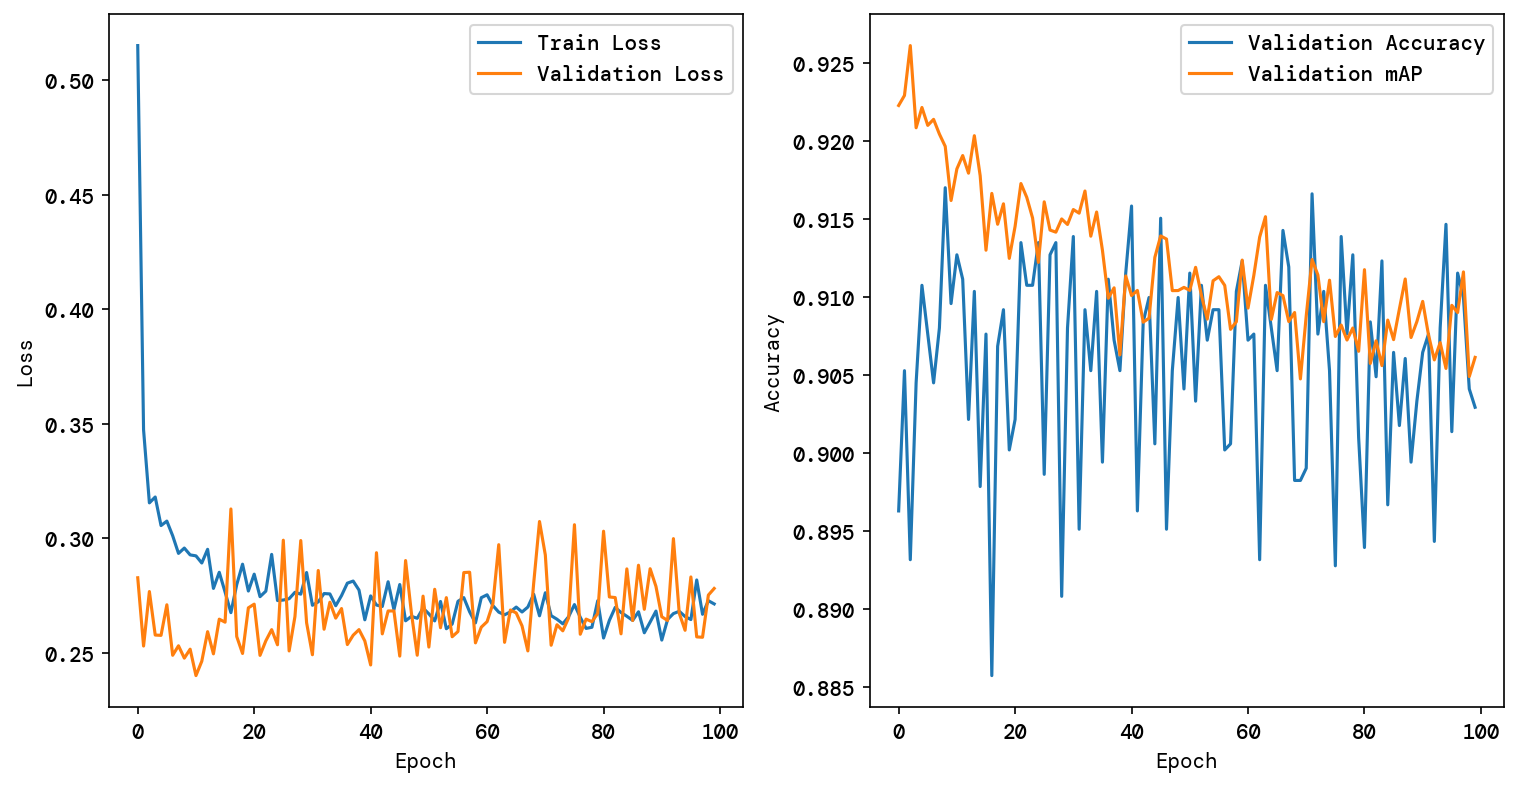
\includegraphics[width=0.8\textwidth]{training.png}
    \caption{Example image}
    \label{fig:training}
\end{figure}
\begin{figure*}[]
    \centering
    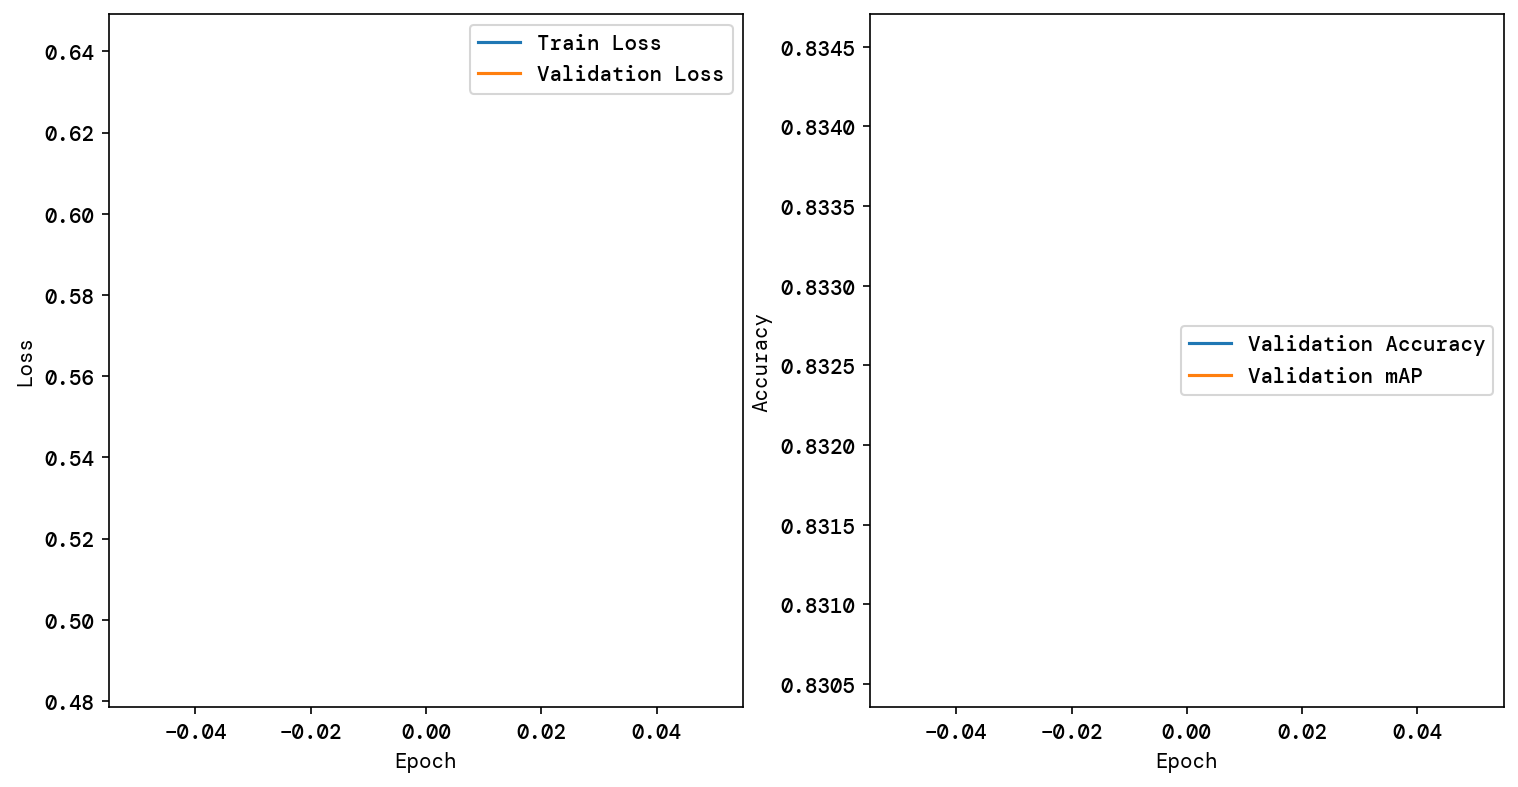
\includegraphics[width=0.8\textwidth]{training_only_freeze_conv.png}
    \caption{Example image}
    \label{fig:training}
\end{figure}

Reported percentage of non-zero activations in the feature maps across 200 images
[0.8, 0.7, 0.6, 0.5, 0.4]

\begin{figure*}[h]
    \centering
    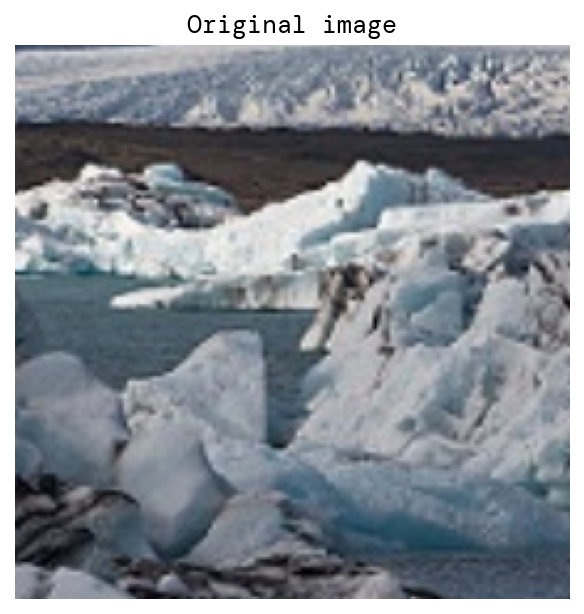
\includegraphics[width=0.4\textwidth]{original-image.png}
    \caption{Example image}
    \label{fig:original-image}
\end{figure}
\begin{figure*}[h]
    \centering
    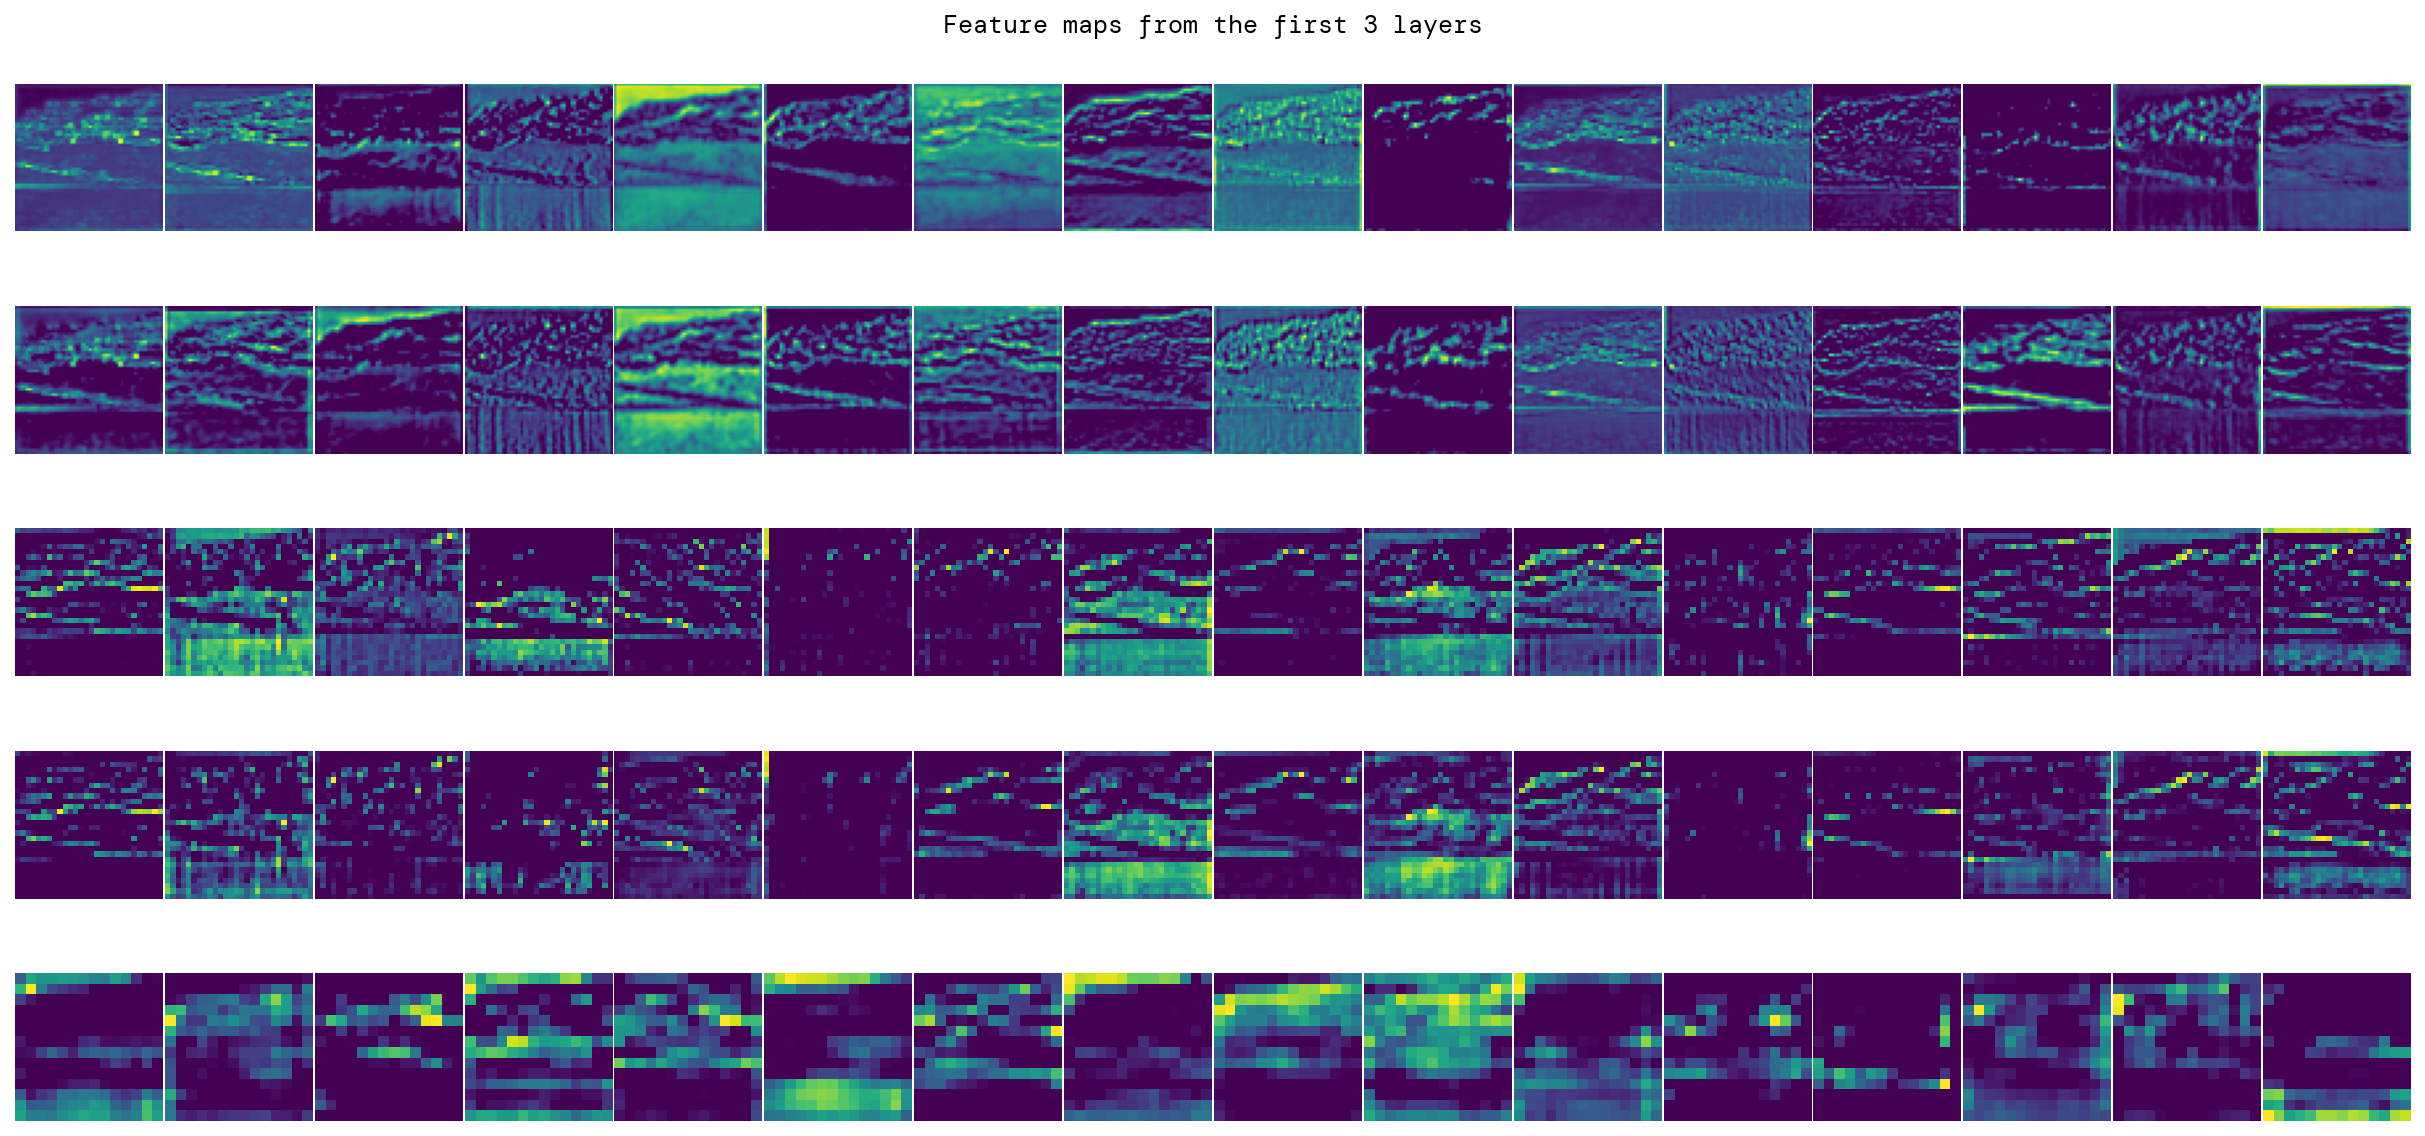
\includegraphics[width=1.0\textwidth]{featuremaps.png}
    \caption{Example image}
    \label{fig:featuremaps}
\end{figure}

\begin{figure*}[h]
    \centering
    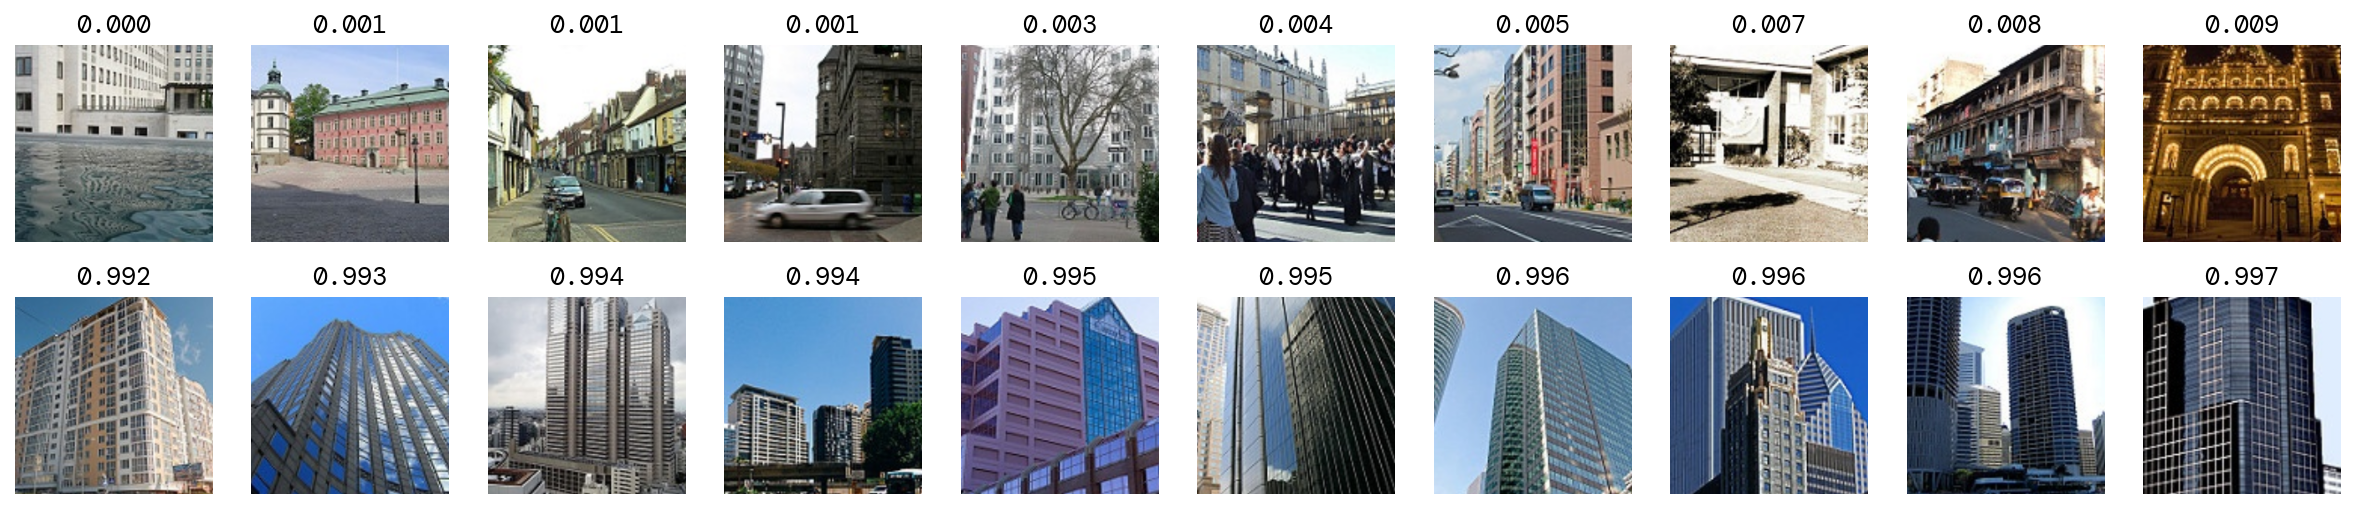
\includegraphics[width=1.0\textwidth]{best_worst_first_class.png}
    \caption{Example image}
    \label{fig:featuremaps}
\end{figure}


\begin{figure*}[h]
    \centering
    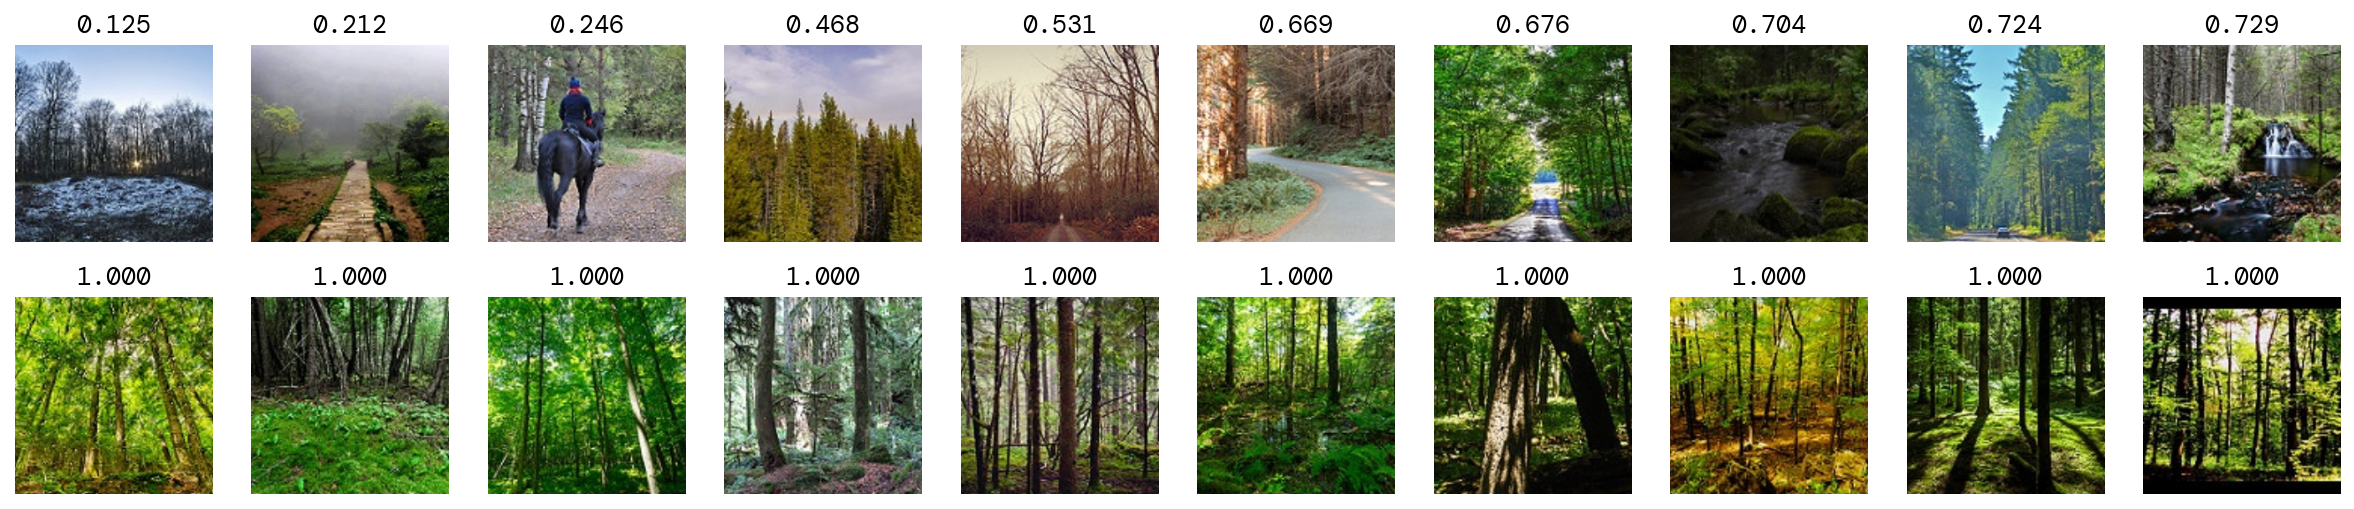
\includegraphics[width=1.0\textwidth]{best_worst_second_class.png}
    \caption{Example image}
    \label{fig:featuremaps}
\end{figure}


\begin{figure*}[h]
    \centering
    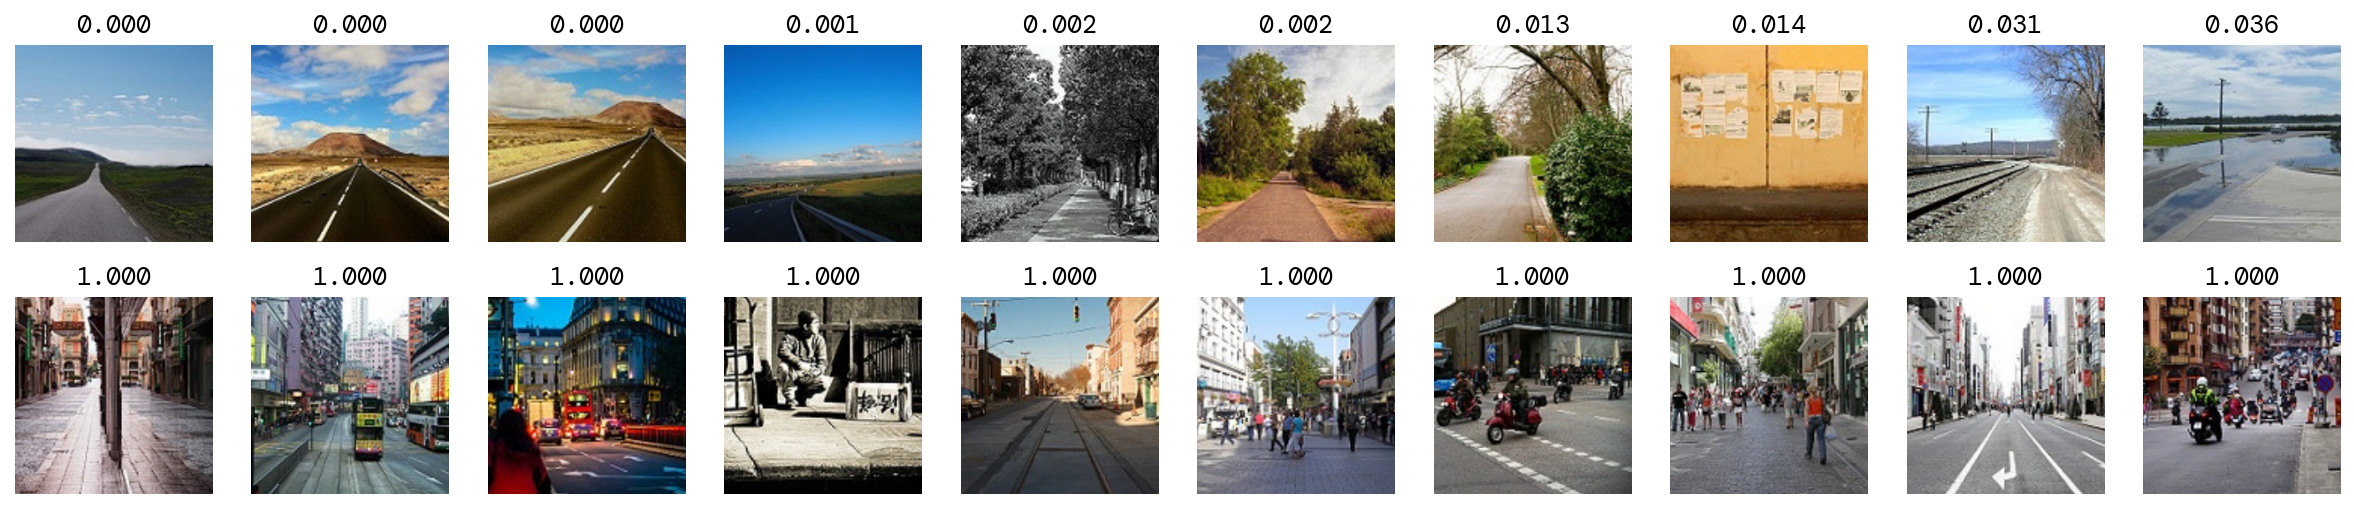
\includegraphics[width=1.0\textwidth]{best_worst_sixth_class.png}
    \caption{Example image}
    \label{fig:featuremaps}
\end{figure}

\end{document}
